\chapter{Resultats}
\label{chap-results}

\paragraph{Structure moléculaire du calcium oxalate}
%TODO add reference
La cellule élémentaire de calcium oxalate ($Ca C_2 O_4$) contient 28 atomes. Il est de structure monoclique et de groupe de symétrie $P2/m$ ($\#$10) (cf. \cref{BrillouinZone})
%TODO add bilbao

\begin{figure}[!h]\label{BrillouinZone}
    \centering
    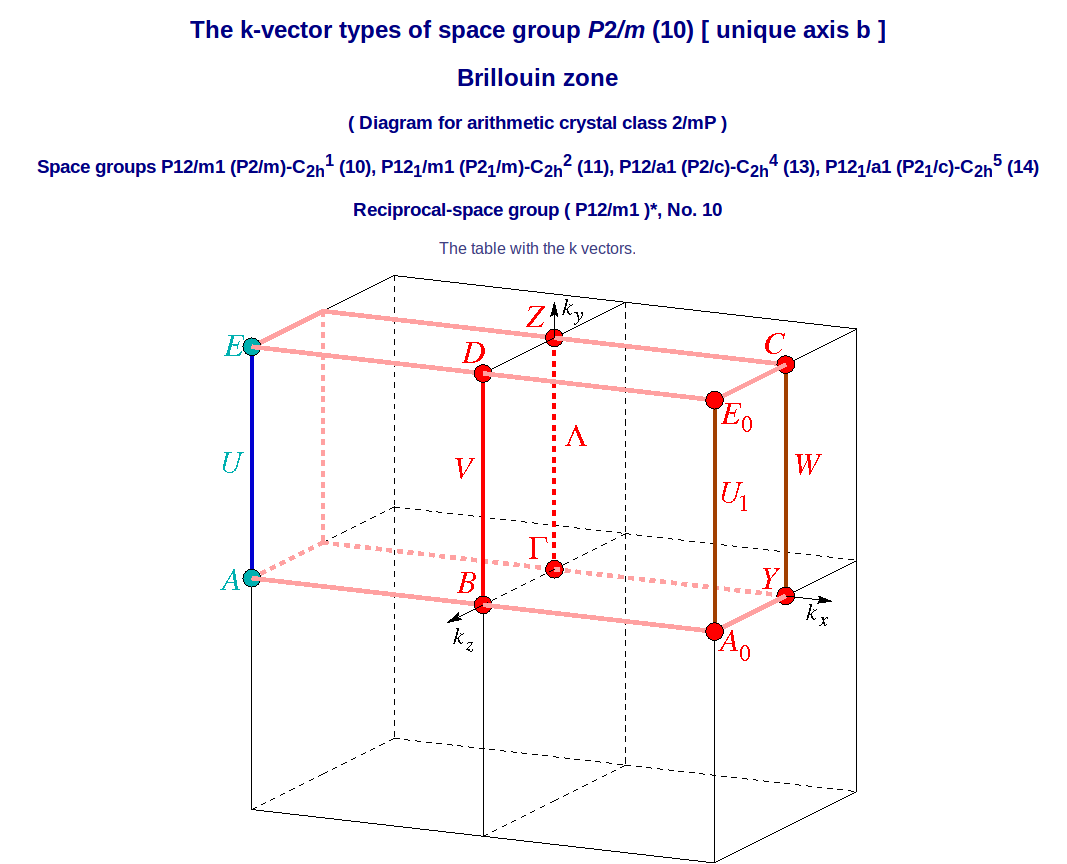
\includegraphics[width=8cm]{BrillouinZone}
    \caption{aldarpa}
\end{figure}
%%%%%%%%%%%%%%%%%%%%%%%%%%%%%%%%%%%%%%%%%
\paragraph{Ecut}
Pour commencer, on étudie la convergence du calcul de l'état fondamental de calcium oxalate. On fait varier le seuil d'énergie $E_{cut}$ entre 20 et 100 Hatree.
On constate que pour tous ces seuils d'énergies, on obtient bien une convergence au bout de 15 itérations. La relation entre l'énergie totale du système à la convergence en fonction de l'énergie de seuil est tracée dans la \cref{Ecut}.
À partir de $E_{cut} = 40$ Hatree, l'énergie totale du système est bien minimisée. On choisit donc cette énergie de seuil pour la suite du calcul de l'état fondamental.

\begin{figure}[!h]\label{Ecut}
    \centering
    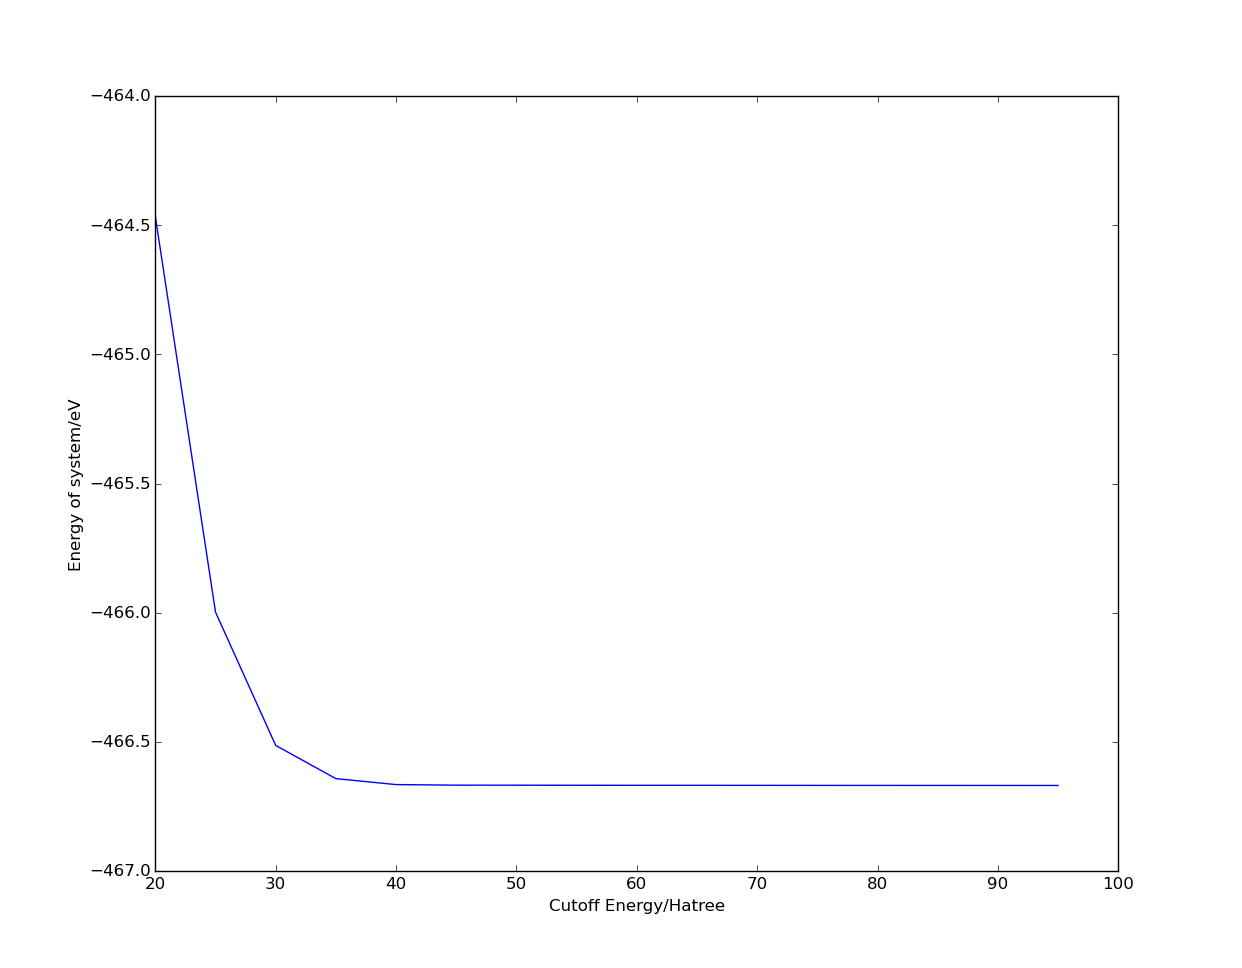
\includegraphics[width=8cm]{E_cut}
    \caption{Ecut}
\end{figure}

%TODO ajouter la structure de bandes

Dans un premier temps, avant de passer à l'état exicité, on peut construire sa structure de bandes à l'aide du calcul d'Abinit (cf. \cref{BrillouinZone}).
Il est à remarquer que la structure de bande des états exicités seront différents que celle de l'état fondamental.
Cependant, on pourrait avoir des idées sur celle des états excités.
Notamment, le gap de la structure de bande montre que le calcium oxalate n'est pas un conducteur.
Par ailleurs, comme le gap n'est pas direct, on peut donc observer des lumières émises dans des directions non parallèles à la lumière incidente.

%%%%%%%%%%%%%%%%%%%%%%%%%%%%%%%%%%%%%%%%%%%%%%

\paragraph{rpa kpt compare}
On crée des fichiers décrivant la fonction d'onde de l'état fondamental avec des échantillonnages de la première zone de Brillouin différents, où dans la première zone de Brouillin, il y a respectivement 16, 120 et 480 points-k.
La motivation est de pouvoir avoir un échantillonnage assez fin pour obtenir tous les états d'excitation possibles sans avoir trop de points-k, ce qui demandera un temps de calcul considérable.
%TODO verifier si les parametres sont bien mentionnes auparavant
Pour connaître le meilleur échantillonnage à utiliser à notre disposition, on fait d'abord les calculs en prenant RPA (ramdom phase approximation) comme méthode d'approximation du terme d'échange et de corrélation.
Les résultats sont montrés dans la \cref{kptCompare}.
On peut remarquer que les résultats pour 120 points-k et pour 480 points-k sont quasiment identiques en basses énergies ($<$ 20 eV).
On choisit donc l'échantillonnage de 120 points-k pour continuer.

\begin{figure}[!h]\label{kptCompare}
    \centering
    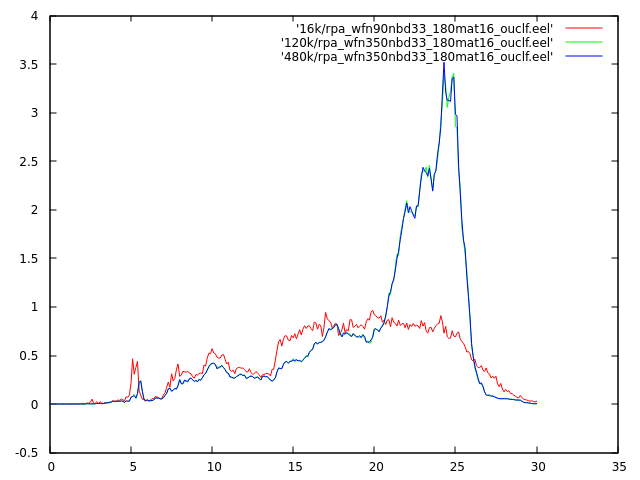
\includegraphics[width=8cm]{rpa_kpt_compare}
    \caption{rpa}
\end{figure}

%%%%%%%%%%%%%%%%%%%%%%%%%%%%%%%%%%%%%%%%%%%%%%%%%%%%%%%%%%%%%%%
\paragraph{alda vs rpa}\label{aldaRPA}
La méthode d'approximation RPA prend moins de temps pour le calcul mais pourrait perdre la précision. Il est donc judicieux de comparer les résultats obtenus en appliquant RPA avec ceux obtenus en appliquant ALDA (adiabatic local density approximation).
Les deux approximations nous donnent des résultats assez proches en basses énergies.
Dans le cadre de ce projet, on se contente d'étudier les caractéristiques de calcium oxalate en basses énergie en raison du délai.
Il est donc tout à fait pertinent de faire notre calcul en RPA pour gagner en temps de calcul.
\begin{figure}[!h]
    \centering
    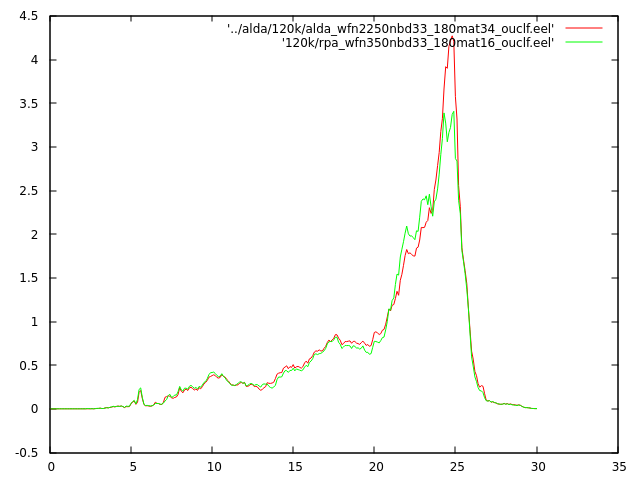
\includegraphics[width=8cm]{alda_vs_rpa}
    \caption{alda}
\end{figure}
%%%%%%%%%%%%%%%%%%%%%%%%%%%%%%%%%%%%%%%%%%%%%%%%%%%%%%%555555555%%%%%


\begin{figure}[!h]\label{CVwfnshRPA}
    \centering
    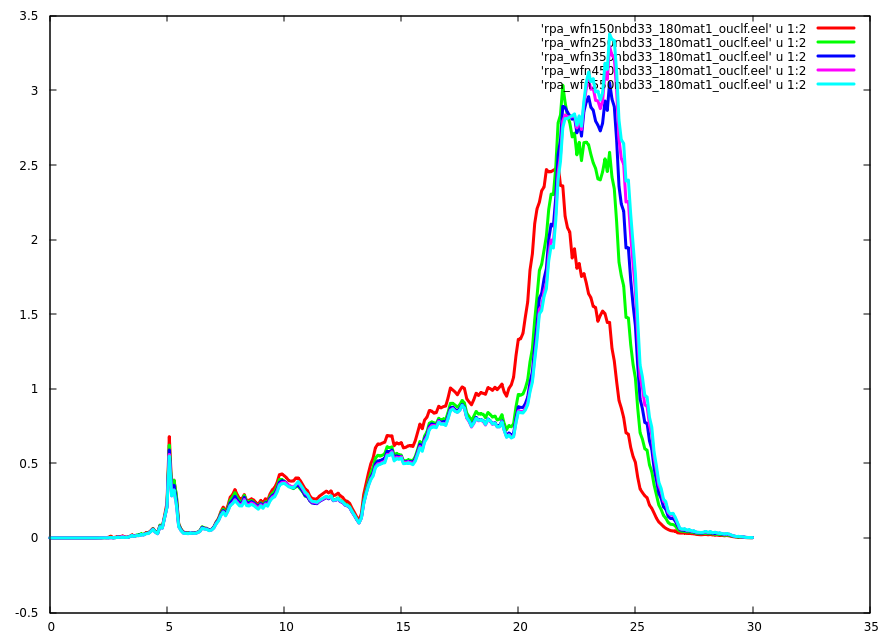
\includegraphics[width=8cm]{cv_wfnsh_rpa}
    \caption{convergence wfnsh rpa}
\end{figure}

\paragraph{q6}
\begin{figure}[!h]
    \centering
    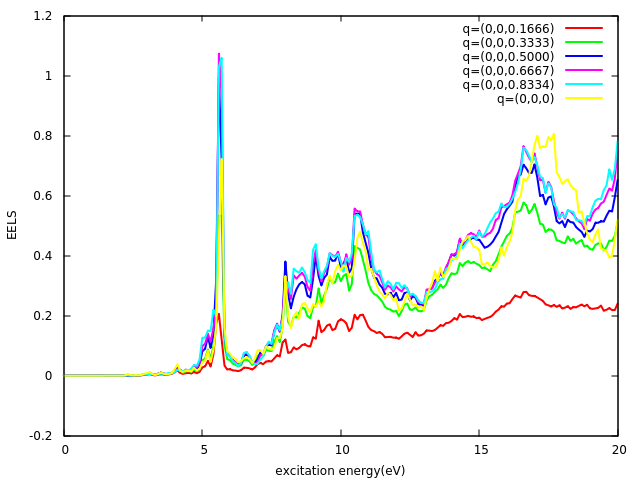
\includegraphics[width=8cm]{q6}
    \caption{q = (0, 0, 0.6)}
\end{figure}


\paragraph{q8}
\begin{figure}[!h]
    \centering
    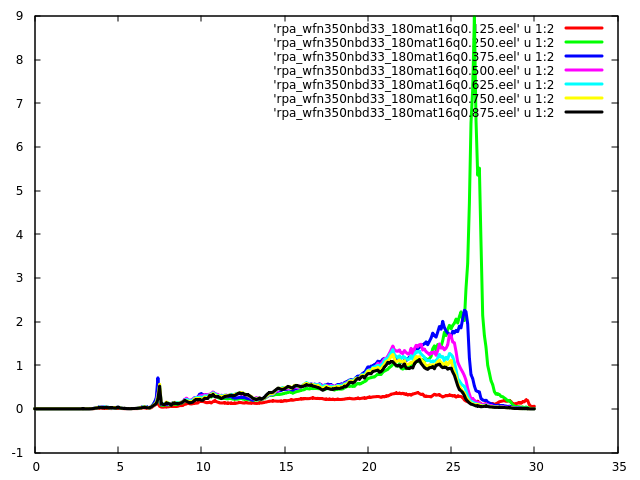
\includegraphics[width=8cm]{q8}
    \caption{q = (0, 0.125, 0)}
\end{figure}


\paragraph{q10}
\begin{figure}[!h]
    \centering
    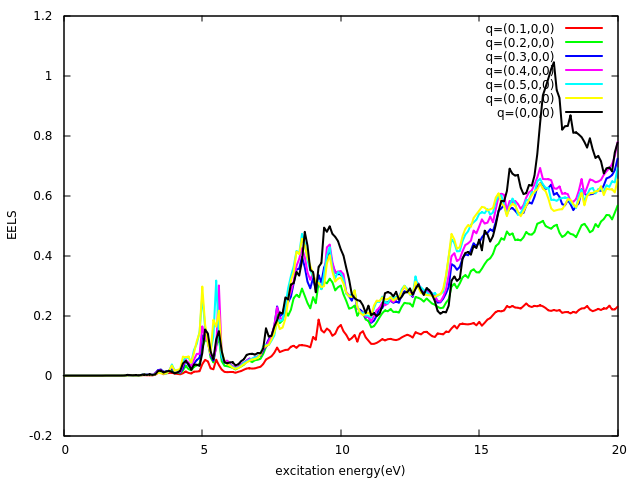
\includegraphics[width=8cm]{q10}
    \caption{q = (0.1, 0, 0)}
\end{figure}
